\documentclass{standalone}
\usepackage{tikz}
\usetikzlibrary{patterns, positioning}
\usepackage[sfdefault]{ClearSans} %% option 'sfdefault' activates Clear Sans as the default text font
\usepackage[T1]{fontenc}

\begin{document}
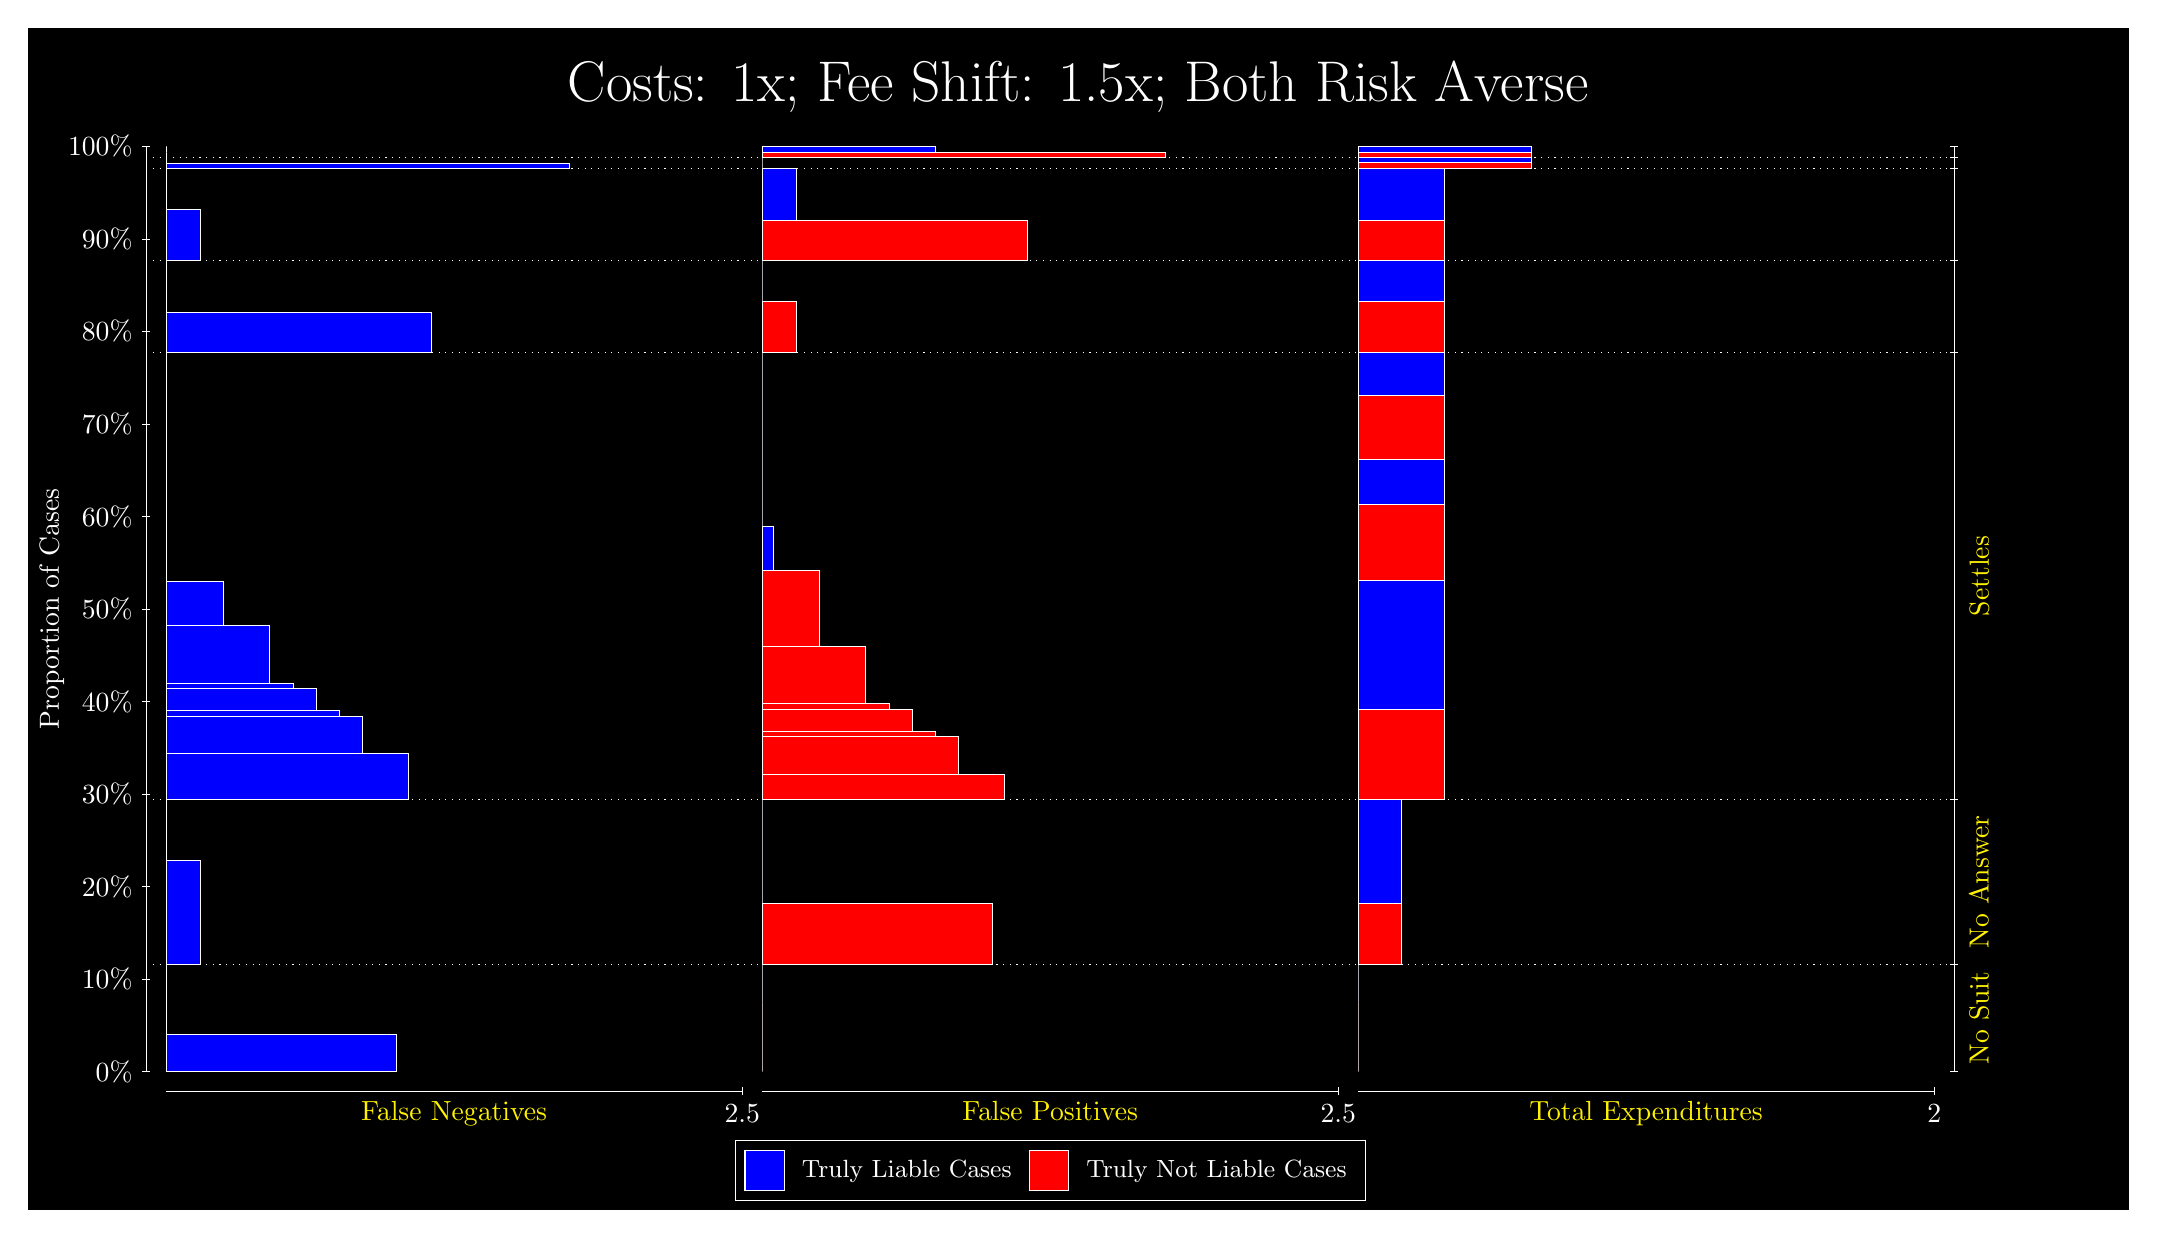
\begin{tikzpicture}
\draw[fill=black] (0,0) rectangle (26.667,15);
\draw[text=white] (0,13.5) rectangle (26.667,15) node[midway] {\huge Costs: 1x; Fee Shift: 1.5x; Both Risk Averse};
\draw[white, very thin] (1.5,1.75) -- (1.5,13.5);
\node[rotate=90, text=white, anchor=center] at (0.3, 7.625) {Proportion of Cases};
\draw[white, very thin] (1.45,1.75) -- (1.55,1.75);
\node[text=white, anchor=east] at (1.45, 1.75) {0\%};
\draw[white, very thin] (1.45,2.925) -- (1.55,2.925);
\node[text=white, anchor=east] at (1.45, 2.925) {10\%};
\draw[white, very thin] (1.45,4.1) -- (1.55,4.1);
\node[text=white, anchor=east] at (1.45, 4.1) {20\%};
\draw[white, very thin] (1.45,5.275) -- (1.55,5.275);
\node[text=white, anchor=east] at (1.45, 5.275) {30\%};
\draw[white, very thin] (1.45,6.45) -- (1.55,6.45);
\node[text=white, anchor=east] at (1.45, 6.45) {40\%};
\draw[white, very thin] (1.45,7.625) -- (1.55,7.625);
\node[text=white, anchor=east] at (1.45, 7.625) {50\%};
\draw[white, very thin] (1.45,8.8) -- (1.55,8.8);
\node[text=white, anchor=east] at (1.45, 8.8) {60\%};
\draw[white, very thin] (1.45,9.975) -- (1.55,9.975);
\node[text=white, anchor=east] at (1.45, 9.975) {70\%};
\draw[white, very thin] (1.45,11.15) -- (1.55,11.15);
\node[text=white, anchor=east] at (1.45, 11.15) {80\%};
\draw[white, very thin] (1.45,12.325) -- (1.55,12.325);
\node[text=white, anchor=east] at (1.45, 12.325) {90\%};
\draw[white, very thin] (1.45,13.5) -- (1.55,13.5);
\node[text=white, anchor=east] at (1.45, 13.5) {100\%};

\draw[white, very thin] (24.457,1.75) -- (24.457,13.5);
\draw[white, very thin] (24.407,1.75) -- (24.507,1.75);
\node[anchor=west] at (24.407, 1.75) {};
\draw[white, very thin] (24.407,3.1071) -- (24.507,3.1071);
\node[anchor=west] at (24.407, 3.1071) {};
\draw[white, very thin] (24.407,5.2071) -- (24.507,5.2071);
\node[anchor=west] at (24.407, 5.2071) {};
\draw[white, very thin] (24.407,10.88) -- (24.507,10.88);
\node[anchor=west] at (24.407, 10.88) {};
\draw[white, very thin] (24.407,12.05) -- (24.507,12.05);
\node[anchor=west] at (24.407, 12.05) {};
\draw[white, very thin] (24.407,13.218) -- (24.507,13.218);
\node[anchor=west] at (24.407, 13.218) {};
\draw[white, very thin] (24.407,13.359) -- (24.507,13.359);
\node[anchor=west] at (24.407, 13.359) {};
\draw[white, very thin] (24.407,13.5) -- (24.507,13.5);
\node[anchor=west] at (24.407, 13.5) {};

\draw[white, very thin, fill=blue] (1.75,1.75) rectangle (4.6775,2.2283);
\draw[white, very thin, fill=red] (1.75,2.2283) rectangle (1.75,3.1071);
\draw[white, very thin, fill=blue] (1.75,3.1071) rectangle (2.1891,4.4295);
\draw[white, very thin, fill=red] (1.75,4.4295) rectangle (1.75,5.2071);
\draw[white, very thin, fill=blue] (1.75,5.2071) rectangle (4.8239,5.7859);
\draw[white, very thin, fill=blue] (1.75,5.7859) rectangle (4.2384,6.268);
\draw[white, very thin, fill=blue] (1.75,6.268) rectangle (3.9457,6.3337);
\draw[white, very thin, fill=blue] (1.75,6.3337) rectangle (3.6529,6.6129);
\draw[white, very thin, fill=blue] (1.75,6.6129) rectangle (3.3602,6.6854);
\draw[white, very thin, fill=blue] (1.75,6.6854) rectangle (3.0674,7.4177);
\draw[white, very thin, fill=blue] (1.75,7.4177) rectangle (2.4819,7.9715);
\draw[white, very thin, fill=red] (1.75,7.9715) rectangle (1.75,10.88);
\draw[white, very thin, fill=blue] (1.75,10.88) rectangle (5.1167,11.395);
\draw[white, very thin, fill=red] (1.75,11.395) rectangle (1.75,12.05);
\draw[white, very thin, fill=blue] (1.75,12.05) rectangle (2.1891,12.704);
\draw[white, very thin, fill=red] (1.75,12.704) rectangle (1.75,13.218);
\draw[white, very thin, fill=blue] (1.75,13.218) rectangle (6.8732,13.281);
\draw[white, very thin, fill=red] (1.75,13.281) rectangle (1.75,13.359);
\draw[white, very thin, fill=red] (1.75,13.359) rectangle (1.75,13.422);
\draw[white, very thin, fill=blue] (1.75,13.422) rectangle (1.75,13.5);
\draw[white, very thin, fill=red] (9.3189,1.75) rectangle (9.3189,2.6289);
\draw[white, very thin, fill=blue] (9.3189,2.6289) rectangle (9.3189,3.1071);
\draw[white, very thin, fill=red] (9.3189,3.1071) rectangle (12.246,3.8847);
\draw[white, very thin, fill=blue] (9.3189,3.8847) rectangle (9.3189,5.2071);
\draw[white, very thin, fill=red] (9.3189,5.2071) rectangle (12.393,5.5235);
\draw[white, very thin, fill=red] (9.3189,5.5235) rectangle (11.807,6.0056);
\draw[white, very thin, fill=red] (9.3189,6.0056) rectangle (11.515,6.0713);
\draw[white, very thin, fill=red] (9.3189,6.0713) rectangle (11.222,6.3505);
\draw[white, very thin, fill=red] (9.3189,6.3505) rectangle (10.929,6.423);
\draw[white, very thin, fill=red] (9.3189,6.423) rectangle (10.636,7.1553);
\draw[white, very thin, fill=red] (9.3189,7.1553) rectangle (10.051,8.1157);
\draw[white, very thin, fill=blue] (9.3189,8.1157) rectangle (9.4652,8.6695);
\draw[white, very thin, fill=blue] (9.3189,8.6695) rectangle (9.3189,10.88);
\draw[white, very thin, fill=red] (9.3189,10.88) rectangle (9.758,11.535);
\draw[white, very thin, fill=blue] (9.3189,11.535) rectangle (9.3189,12.05);
\draw[white, very thin, fill=red] (9.3189,12.05) rectangle (12.686,12.564);
\draw[white, very thin, fill=blue] (9.3189,12.564) rectangle (9.758,13.218);
\draw[white, very thin, fill=red] (9.3189,13.218) rectangle (9.3189,13.295);
\draw[white, very thin, fill=blue] (9.3189,13.295) rectangle (9.3189,13.359);
\draw[white, very thin, fill=red] (9.3189,13.359) rectangle (14.442,13.422);
\draw[white, very thin, fill=blue] (9.3189,13.422) rectangle (11.515,13.5);
\draw[white, very thin, fill=red] (16.888,1.75) rectangle (16.888,2.6289);
\draw[white, very thin, fill=blue] (16.888,2.6289) rectangle (16.888,3.1071);
\draw[white, very thin, fill=red] (16.888,3.1071) rectangle (17.437,3.8847);
\draw[white, very thin, fill=blue] (16.888,3.8847) rectangle (17.437,5.2071);
\draw[white, very thin, fill=red] (16.888,5.2071) rectangle (17.986,6.3505);
\draw[white, very thin, fill=blue] (16.888,6.3505) rectangle (17.986,7.9884);
\draw[white, very thin, fill=red] (16.888,7.9884) rectangle (17.986,8.9488);
\draw[white, very thin, fill=blue] (16.888,8.9488) rectangle (17.986,9.5276);
\draw[white, very thin, fill=red] (16.888,9.5276) rectangle (17.986,10.332);
\draw[white, very thin, fill=blue] (16.888,10.332) rectangle (17.986,10.88);
\draw[white, very thin, fill=red] (16.888,10.88) rectangle (17.986,11.535);
\draw[white, very thin, fill=blue] (16.888,11.535) rectangle (17.986,12.05);
\draw[white, very thin, fill=red] (16.888,12.05) rectangle (17.986,12.564);
\draw[white, very thin, fill=blue] (16.888,12.564) rectangle (17.986,13.218);
\draw[white, very thin, fill=red] (16.888,13.218) rectangle (19.083,13.295);
\draw[white, very thin, fill=blue] (16.888,13.295) rectangle (19.083,13.359);
\draw[white, very thin, fill=red] (16.888,13.359) rectangle (19.083,13.422);
\draw[white, very thin, fill=blue] (16.888,13.422) rectangle (19.083,13.5);
\draw[white, dotted] (1.5,3.1071) -- (24.457,3.1071);
\draw[white, dotted] (1.5,5.2071) -- (24.457,5.2071);
\draw[white, dotted] (1.5,10.88) -- (24.457,10.88);
\draw[white, dotted] (1.5,12.05) -- (24.457,12.05);
\draw[white, dotted] (1.5,13.218) -- (24.457,13.218);
\draw[white, dotted] (1.5,13.359) -- (24.457,13.359);
\draw[white, very thin] (1.75,1.5) -- (9.0689,1.5);
\node[text=yellow, anchor=north] at (5.4094, 1.5) {False Negatives};
\draw[white, very thin] (9.0689,1.45) -- (9.0689,1.55);
\node[text=white, anchor=north] at (9.0689, 1.45) {2.5};

\draw[white, very thin] (9.3189,1.5) -- (16.638,1.5);
\node[text=yellow, anchor=north] at (12.978, 1.5) {False Positives};
\draw[white, very thin] (16.638,1.45) -- (16.638,1.55);
\node[text=white, anchor=north] at (16.638, 1.45) {2.5};

\draw[white, very thin] (16.888,1.5) -- (24.207,1.5);
\node[text=yellow, anchor=north] at (20.547, 1.5) {Total Expenditures};
\draw[white, very thin] (24.207,1.45) -- (24.207,1.55);
\node[text=white, anchor=north] at (24.207, 1.45) {2};

\node[text=yellow, centered, rotate=90] at (24.777, 2.4286) {No Suit};
\node[text=yellow, centered, rotate=90] at (24.777, 4.1571) {No Answer};
\node[text=yellow, centered, rotate=90] at (24.777, 8.0436) {Settles};





\draw (12.978300999999998,1.5) node[draw=none] (baseCoordinate) {};
\begin{scope}[align=center]
        \matrix[scale=0.5, draw=white, below=0.5cm of baseCoordinate, nodes={draw}, column sep=0.1cm]{
            \node[rectangle, draw, minimum width=0.5cm, minimum height=0.5cm, fill=blue] {}; &
            \node[draw=none, font=\small, text=white] (B) {Truly Liable Cases}; &
            \node[rectangle, draw, minimum width=0.5cm, minimum height=0.5cm, fill=red] {}; &
            \node[draw=none, font=\small, text=white] (B) {Truly Not Liable Cases}; \\
            };
\end{scope}

\end{tikzpicture}
\end{document}